\documentclass[twoside,twocolumn]{article}

\usepackage{blindtext} % Package to generate dummy text throughout this template 
\usepackage{graphicx}
\usepackage[sc]{mathpazo} % Use the Palatino font
\usepackage[T1]{fontenc} % Use 8-bit encoding that has 256 glyphs
\linespread{1.05} % Line spacing - Palatino needs more space between lines
\usepackage{microtype} % Slightly tweak font spacing for aesthetics

\usepackage[english]{babel} % Language hyphenation and typographical rules

\usepackage[hmarginratio=1:1,top=32mm,columnsep=20pt]{geometry} % Document margins
\usepackage[hang, small,labelfont=bf,up,textfont=it,up]{caption} % Custom captions under/above floats in tables or figures
\usepackage{booktabs} % Horizontal rules in tables
\usepackage{graphicx}
\usepackage{lettrine} % The lettrine is the first enlarged letter at the beginning of the text

\usepackage{enumitem} % Customized lists
\setlist[itemize]{noitemsep} % Make itemize lists more compact

\usepackage{abstract} % Allows abstract customization
\renewcommand{\abstractnamefont}{\normalfont\bfseries} % Set the "Abstract" text to bold
\renewcommand{\abstracttextfont}{\normalfont\small\itshape} % Set the abstract itself to small italic text

\usepackage{titlesec} % Allows customization of titles

\titleformat{\section}[block]{\large\scshape\centering}{\thesection.}{1em}{} % Change the look of the section titles
\titleformat{\subsection}[block]{\large}{\thesubsection.}{1em}{} % Change the look of the section titles

\usepackage{fancyhdr} % Headers and footers
\pagestyle{fancy} % All pages have headers and footers
\fancyhead{} % Blank out the default header
\fancyfoot{} % Blank out the default footer
\fancyhead[C]{Comparative Datawarehouse vs Datalake $\bullet$ Julio 2022 $\bullet$ } % Custom header text
\fancyfoot[RO,LE]{\thepage} % Custom footer text

\usepackage{titling} % Customizing the title section

\usepackage{hyperref} % For hyperlinks in the PDF

%----------------------------------------------------------------------------------------
%	TITLE SECTION
%----------------------------------------------------------------------------------------
\providecommand{\keywords}[1]{
  \small	
  \textbf{\textit{\quad \quad Keywords: }} #1}

\providecommand{\pclave}[1]{
  \small	
  \textbf{\textit{\quad \quad Palabras Clave: }} #1}

%Idiomas: \selectlanguage{english} \selectlanguage{spanish}

\begin{document}

\title{Trabajo Encargado 03: Comparative Datawarehouse vs Datalake}

\begin{titlepage}
\begin{figure}[htb]
\begin{center}

\includegraphics[width=5cm]{imagenes/logo.png}
\end{center}
\end{figure}
\vspace*{-0.25in}
\begin{center}
\large{UNIVERSIDAD PRIVADA DE TACNA}\\
\vspace*{-0.025in}
INGENIERIA DE SISTEMAS  \\	

\vspace*{0.5in}
\begin{large}
TITULO:\\
\end{large}

\vspace*{0.1in}
\begin{Large}
\textbf{ Comparative Datawarehouse vs Datalake} \\
\end{Large}

\vspace*{0.3in}
\begin{Large}
\textbf{CURSO:} \\
\end{Large}

\vspace*{0.1in}
\begin{large}
Inteligencia de Negocios\\
\end{large}

\vspace*{0.3in}
\begin{Large}
\textbf{DOCENTE:} \\
\end{Large}

\vspace*{0.1in}
\begin{large}
 Ing. Patrick Cuadros Quiroga\\
\end{large}

\vspace*{0.2in}
\vspace*{0.1in}
\begin{large}

Integrantes: \\
\begin{flushleft}
Maldonado Cancapi, Carlos Alejandro\hfill(2018000660) \\
Huillca Aroni, Alfredo\hfill(2018060903)\\
Anahua Huayhua, Jenny Karen\hfill(2018062150)\\
Coloma Colquehuanca, Kiara\hfill(2018062218)\\

\end{flushleft}
\end{large}

\vspace*{0.1in}
\begin{large}
Tacna - Perú\\
2022
\end{large}
\end{center}
\end{titlepage}

\setlength{\droptitle}{-4\baselineskip} % Move the title up

\pretitle{\begin{center}\Huge\bfseries} % Article title formatting
\posttitle{\end{center}} % Article title closing formatting
\title{MLOps} % Article title

\date{\today} % Leave empty to omit a date                     
\renewcommand{\maketitlehookd}{%

}

%----------------------------------------------------------------------------------------



% Print the title
\maketitle

%----------------------------------------------------------------------------------------
%	ARTICLE CONTENTS
%----------------------------------------------------------------------------------------

\section{Resumen}
Machine Learning Model Operationalization Management (MLOps) 
constituye una metodología de trabajo orientada al desarrollo 
de modelos de predicción basados en algoritmos de Machine Learning. 
Esta metodología está conformada por un conjunto exhaustivo de 
principios, recomendaciones, directrices y buenas prácticas 
enfocadas en el abordaje metodológico del desarrollo de modelos 
de Machine Learning desde su experimentación inicial hasta su 
puesta en producción. Para alcanzar este objetivo, esta 
metodología propone una división del desarrollo de estos 
proyectos en 4 fases consecutivas. Estas fases comprenden las 
tareas de desarrollo de modelos, preparación de los modelos para 
el despliegue en producción, el despliegue en producción y la 
monitorización de los modelos desplegados.
%------------------------------------------------

\section{Abstract}

Machine Learning Model Operationalization Management
(MLOps) constitutes a work methodology
oriented to the development of prediction models
based on Machine Learning algorithms.
This methodology is made up of a set
comprehensive list of principles, recommendations,
guidelines and good practices focused
in the methodological approach to development
of Machine Learning models from your
initial experimentation until its commissioning
production. To reach this goal,
This methodology proposes a division of the
development of these projects in 4 phases
consecutive. These phases include
model development tasks, preparation
of the models for deployment in production,
production deployment and monitoring
of the deployed models.





%------------------------------------------------
\section{Introduccion}
En la actualidad, las técnicas y 
herramientas de Machine Learning 
(conocido como Aprendizaje Automático en español)
 están siendo adoptadas en la práctica totalidad 
 de industrias y disciplinas; sin embargo, más de 
 la mitad de los análisis estadísticos y modelos de 
 Machine Learning creados por las organizaciones nunca 
 llegan a desplegarse en producción. La puesta en producción 
 de los modelos de predicción experimentales desarrollados por 
 investigadores o científicos de datos constituye un desafío 
 técnico en el que están involucrados diversos campos y disciplinas 
 de las ciencias de la computación. Un desafío que, frecuentemente, 
 no se aborda con éxito. Actualmente existen avanzadas y potentes 
 herramientas de Machine Learning que permiten la construcción de 
 sistemas complejos con gran rapidez. Sin embargo, estos desarrollos 
 acelerados de modelos de Machine Learning suelen acarrear una gran 
 deuda técnica (Sculley et al., 2014) que las organizaciones tendrán 
 que asumir a la hora de implementar estos modelos como sistemas 
 preparados para dar servicio a gran escala de forma fiable y
 automatizada. A raíz de la necesidad de solventar estas dificultades 
 han surgido, durante los últimos años, diversas disciplinas y 
 metodologías enfocadas en la disminución de la deuda técnica y 
 la estandarización del ciclo de vida del desarrollo de proyectos 
 basados en Machine Learning. Estos principios se engloban en el 
 denominado Machine Learning Model Operationalization Management 
 (MLOps), un concepto de muy reciente aparición que está rápidamente 
 empezando a constituir un componente crítico en el desarrollo y 
 despliegue exitoso de los modelos de Machine Learning (Visengeriyeva 
 et al., s.f.).
\begin{center}

\end{center}

\section{Desarrollo}

\subsection{MLOps}
\subsubsection{Concepto}
MLOps es una extension de la metodologia DevOps que busca incluir activos 
de aprendizaje automatico y ciencia de datos como ciudadanos de primera clase dentro de la 
ecologia DevOps. Dentro de MLOps existen tres niveles de implementacion de 
Machine Learnign
\begin{itemize}
    \item Data: datos,fase, ingestion, curado, etc.
    \item Model: testing, evaluacion de los modelos, empaquetado y como se van a desplegar
    \item Code: el codigo, donde se ejecuta todo el modelo en sí.
\end{itemize}
El nombre de MLOps y su definición están basados ampliamente en el concepto de DevOps (Atlassian, s.f.), una disciplina muy extendida y generalizada que tiene como objetivo la estandarización del proceso de desarrollo de software y su integración, actualización y despliegue. Aunque similares en objeto, DevOps no puede ser directamente aplicado a los proyectos de Machine Learning. Este impedimento tiene su origen en la naturaleza dinámica y mutable de los datos, que cambian junto al fenómeno del mundo físico que se desea modelar. Existe, por tanto, la necesidad de adaptar continuamente los modelos desarrollados para reflejar estos cambios en los datos disponibles. DevOps aborda el desarrollo de proyectos con un código que permanece estático una vez desplegado y, por tanto, no abarca el desarrollo de proyectos que, además de código, también están basados en datos. MLOps surge para suplir estas carencias.
\subsubsection{CICLO DE VIDA}
MLOps establece una metodología aplicada a los proyectos de Machine Learning abordando íntegramente sus fases de desarrollo:

\begin{itemize}
    \item  El desarrollo y entrenamiento de modelos.
    \item  La preparación del modelo para su puesta en producción.
    \item  La puesta en producción del modelo.
    \item  La monitorización y reentrenamiento de modelos.
\end{itemize}


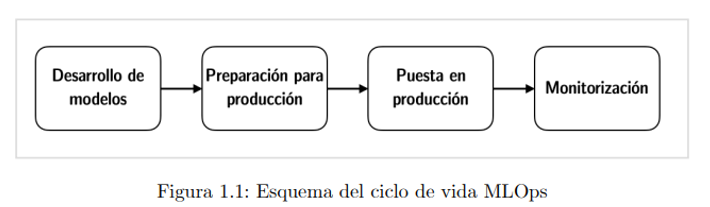
\includegraphics[width=7cm]{imagenes/imagen1.png}
\subsubsection{¿Por qué empezar a aplicar MLOps?}
En la actualidad, nos encontramos en un mundo orientado a datos, que esta vinculado a la cantidad exponencialmente
creciente de los mismos, recogidos digitalmente. Además, nos encontramos con la ascendente importancia de la inteligencia 
Artificial y la Ciencia de Datos, que se deriva de esta tremenda cantidad de informacion generada.

Dependiendo de todos ellos, se pueden explotar de formas distintas, distinguiendo en capacidades(percepcion, cognitivo y aprendizaje) y casos de uso
(vision, audio, voz y lenguaje natural).

\paragraph{¿Que debo tener en cuenta para usar MLOps?}
\begin{itemize}
    \item  Calidad de los datos: tener en cuenta de donde vienen, calidad, si son fiables, etc.
    \item  Degradacion de los modelos: al cabo del tiempo van perdiendo calidad.
    \item  Localidad: en el momento de la preparacion se estan entrenando los modelos con unos datos especificos basados en una geografía.
\end{itemize}


\subsection{Principios MLOps}
\paragraph{Automatización}
El nivel de automatizacion d elas canalizaciones de datos, modelo de ML y código determina la madurez del 
proceso de ML. Con una mayor madurez, tambien aumenta la velocidad para el entrenamiento de nuevos modelos. El 
objetivo de un equipo de MLOps es automatizar la implementacion de modelos de ML en el sistema de software central o como componente de servicio.

Para adoptar MLOps, vemos tres niveles de automatizacion:
\begin{itemize}
    \item  Proceso manual.
    \item  Automatizacion de canalizaciones de aprendizaje automático.
    \item  Automatizacion de canalizacion de CI/CD.
\end{itemize}

\subsection{Continua X}
MLOps es una cultura de ingeniería de ML que incluye las siguientes prácticas:  
\begin{itemize}
    \item  La integracion continua (CI) amplia el codigo y los componentes de prueba y validacion al agregar datos y modelos de prueba y validación.
    \item  La entrega continua (CD) se refiere a la entrega de una canalización de capacitacion de ML que implementa automaticamente otro servicio de predicción del modelo de ML.
    \item  La capacitacion continua (CT) es exclusiva de la propiedad de los sistemas ML, que vuelve a entrenar automaticamente los modelos ML para volver a implementarlos.
    \item  El monitoreo Continuo (CM) se ocupa de monitorear los datos de de produccion y las metricas de rendimiento del modelo, que estan vinculadas a las metricas comerciales.   
\end{itemize}
   

\subsection{Versionado}
El objetivo del control de versiones es tratar los scripts de entrenamiento de ML, los modelos de ML y los conjuntos de datos para el entrenamiento de modelos como cuidadanos de primera clase en los procesados
de DevOps mediante el seguimiento de los modelos de ML y los conjuntos de datos con sistemas de control de versiones.


\subsection{Pruebas}
La tuberia de desarrollo completa incluye tres componentes esenciales, tuberia de datos, tuberia de modelo de ML y tuberia de aplicacion.
De acuerdo con esta separacion, distinguimos tres alcances para las pruebas en los sitemas ML: pruebas de caracteristicas y datos, pruebas para el desarrollo de modelos y pruebas para la infraestructura ML.

\subsection{Vigilancia}
Una vez que se implementó el modelo ML, debe monitorearse para garantizar que el modelo de ML funcione como se esperaba. La siguiente lista de verificacion para las actividades de monitoreo del modelo en produccion se adoptó de 
"La puntuacion de la prueba de ML: una rúbrica para la preparación de la produccion de ML y la reduccion de la deuda tecnica"

\subsection{Reproducibilidad}
La Reproducibilidad en un flujo de trabajo de aprendizaje automatico significa que cada fase del procesamiento de datos,
el entrenamiento del modelo ML y la implementacion del model ML deben producir resultados identicos con la misma entrada.

\subsection{Persona y roles de MLOps}
Un requisito clave para cualquier proceso de MLOps es que satisfaga las necesidades de todos los usuarios del proceso. Para fines de diseño, considere estos usuarios como roles individuales. Para este proyectos,
el equipo identifico los siguentes roles:
\begin{itemize}
    \item Cintifico de datos: crea el modelo de Machine Learning y sus algoritmos.
    \item Ingeniero de datos: Controla el acondicionamiento de datos.
    \item Ingeniero de software: Controla la integracion del modelo en el paquete de recursos y el flijo de trabajo de CI/CD.
    \item Operaciones o TI: supervisa las operaciones del sistema.
    \item Partes interesadas de la empres: se preocupan de las predcciones realizadas por el modelo de Machine Learning y de la ayuda que proporcionan a la empresa.
    \item Usuario final de los datos: Consume la salidad del modelo de forma útil para la toma de decisiones empresariales.  
\end{itemize}
El equipo tenía que abordar tres conclusiones clave de los estudios de roles y funciones:

\begin{itemize}
    \item Los cientificos e ingenierios de datos discrepan en el enfoque y las aptitudes de su trabajo. Facilitar que le cientifico y el ingeniero de datos trabajen en colaboracion es una consideracion importante que tener en cuenta para el diseño del flujo del proceso de MLOps. Requiere nuevas adquisiciones de aptitudes por parte de todos los miembros del equipo.
    \item Exsite un necesidad de unificar todos los roles principales sin apartar a nadie.
    \item Asegurese de entender el modelo conceptual de MLOps.
    \item Llegue a un acuerdo sobre los miembros del equipo que trabajaran juntos.
    \item Establezca las instrucciones de trabajo para lograr objetivos comunes.
    \item Si la parte interesada empresarial y el usuario final de los datos necesitan una manera de interactuar con la salida de datos de los modelos, una interfaz de usuario facil de usar es la solucion estandar.
    \item 
\end{itemize}
Otros equipos experimentaran problemas similares en otros proyectos de aprendizaje automatico a medida que se escalen verticalemnte para su uso en produccion.

\subsection{Arquitectura de la solucion de MLOps}
\includegraphics[width=7cm]{imagenes/imagen2.png}
Los datos proceden de numerosos origines en distintos formatos, por lo qu eestan acondicionados para su insercción en distintos formatos, por lo que estan acondicionados para su insercion en el lago de datos.
El acondicionados para su insercion en el lago de datos. El acondicionamiento se realiza mediante microservicios que funcionan como Azure Functions. Los clientes personalizan los microservicioes para que se ajesten a los orignes de datos y los transforman a un formato CSV normalizado que las canalizaciones de entrenamiento
y puntuacion consumen

\subsection{Arquitectura del sistema}
Existen muchas opciones de diseño disponibles para la arquitectura del sistema.
En el diagrama siguiente se muestra el resultado final del proceso de toma de decisiones que se describe en Guia para la toma de decisiones de Azure Machine Learning para la seleccion optima de herramientas.
\includegraphics[width=7cm]{imagenes/imagen3.png}

\subsection{Arquitectura de procesamiento por lotes}

El aquipo concibio el diseño arquitectonico para admitir un esquema de procesamiento de datos por lotes. Hay alternativas, pero lo que se use debe admitir los procesos de MLOps. El uso completo de los servicios de Azure
disponibles era un requisito de diseño. En el siguiente diagrama se muestra la arquitectura.


\includegraphics[width=7cm]{imagenes/imagen4.png}


\section{Conclusiones}

Los flujos de trabajo de aprendizaje automatico automatizados le permiten reciclar y volver a implementar su modelo.
La integracion continua mantiene el proceso ininterrumpida y mejora continuamente el modelo.
El control de versiones de codigo y datos le permite recrear sus pruebas  y revertir los resultados de produccion a sus cambios originales.
A medida que el aprendizaje automatico crece como dominio, suregiran nuevos sistema que facilitaran a su organizacion la configuracion de MLOps. 

\section{Recomendaciones}
Existen varias plataformas MLOps para administrar el ciclo de vida del aprendizaje automatico. Asegurase de tener en cuenta los factores relevantes al seleccionar la plataforma.


 
 


%----------------------------------------------------------------------------------------
%	REFERENCE LIST
%----------------------------------------------------------------------------------------
\begin{thebibliography}{}

    \bibitem{DOC2008} 
    Ng, A. (n.d.). MLOps: From Model-centric to Data-centric AI. https://www.deeplearning.ai/wp-content/uploads/2021/06/MLOps-From-Model-centric-to-Data-centric-AI.pdf
    \bibitem{FRE2016} 
    Mastering MLops with Dataiku. (n.d.). https://itlligenze.com/uploads/5/137039/files/oreilly-ml-ops.pdf
    \bibitem{FRE2016}
    Kirenz, J., Gröger, C., and Lutsch, A. (n.d.). Retrieved July 4, 2022, from https://www.kirenz.com/slides/data-platform-mlops.pdf
    \bibitem{FRE2019} 
    Georgios Symeonidis, Evangelos Nerantzis, Apostolos Kazakis, and Papakostas (2022). MLOps Definitions, Tools and Challenges ResearchGate unknown https://www.researchgate.net/publication/357552787MLOpsDefinitionsToolsandChallenges
    \bibitem{FRE2019}
    Emilio Fernández Lastra. (2018, October 10). Data Warehouse y Data Lake. Qué son y para qué sirven. Artyco | the Data Driven Company. https://artyco.com/data-warehouse-data-lake-que-es/
    
    \bibitem{FRE2018}
    Por, R., Valderrama, P., Tutorizado, S., Llanos, M., y López. (n.d.). MLOPS para el desarrollo y puesta en producción de modelos de machine learning https://riuma.uma.es/xmlui/bitstream/handle/10630/23550/Valderrama%20Santiago%20Pablo%20Memoria.pdf?sequence=1
   
   \bibitem{FRE2018}
   MLOPS (2022). MLOps Principles https://ml-ops.org/content/mlops-principles
      
   \bibitem{FRE2018}
   MLOps Workload Orchestrator Implementation Guide. (n.d.). Retrieved July 4, 2022, from https://docs.aws.amazon.com/solutions/latest/mlops-workload-orchestrator/mlops-workload-orchestrator.pdf    
    \bibitem{FRE2018}
    MLOps: Continuous Delivery for Machine Learning on AWS. (2020). https://d1.awsstatic.com/whitepapers/mlops-continuous-delivery-machine-learning-on-aws.pdf
	\bibitem{FRE2018}
	Kirenz, J., Gröger, C., y Lutsch, A. (n.d.). Retrieved July 4, 2022, from https://www.kirenz.com/slides/data-platform-mlops.pdf

 
    \end{thebibliography}


%----------------------------------------------------------------------------------------

\end{document}